\documentclass[a4paper,11pt]{article}
\usepackage[czech]{babel}
\usepackage[utf8]{inputenc}
\usepackage[pdftex]{graphicx}
\author{Ondřej Pilát}
\title{Dekodérová deska pro přestavbu platformy MOB pro použití s RaspberryPi}
\begin{document}
\maketitle
\newpage
\tableofcontents
\newpage
\section{Dekodérova deska}
Deska je založena na mikrokontroléru ATMEL Atmega48pa. Mikrokontrolér čte vstupní signály od kvadraturních enkodérů, dekóduje je a~na základě dekódovaného stavu upravuje stav vnitřního 16bit čítače dle směru pohybu enkodérů. 
Připojení signálů a napájení enkodérů je řešeno pomocí dvou postranních zámkových konektorů. Stav čítačů enkodérů lze zjistit komunikací po I2C. 

Případné aktualizace firmwaru mikrokontroléru lze řešit pomocí standardního 6 pinového programovacího konektoru ISP.

Pro testování a ladění má deska k mikrokontroléru připojeno 6 led diod. 

\subsection{Specifikace}
\begin{itemize}
	\item Mikrokontroler Atmega48pa s krystalem 20MHz se zajímavými vlastnostmi jako:
		\begin{itemize}
			\item Flash paměť 4kb
			\item EEPROM 256b
			\item SRAM 512b  
			\item Tři čítače/časovače s porovnávacím módem
			\item Externí přerušení
			\item Komunikace po I2C
			\item Vstupně/výstupní piny
		\end{itemize}
	\item Konektor I2C s~3.3V logikou
	\item Konektor I2C s~5V logikou
	\item 2 konektory pro připojení napájení a signálů kvadraturních enkodérů
	\item 6 pinový standardní konektor ISP pro možnost nahrání nového kódu do mikrokontroléru
	\item 6 diod pro indikaci stavu mikrokontroléru připojených k zemi 
	(svítí při vysoké úrovni na pinech PB0 - PB2 a PD5 - PD7)
	\item Velikost desky 2.25 x 1.35 palců
	\item Rozteč děr je 2.05 x 1.15 palců s a průměr díry 3mm
\end{itemize}

\newpage
\subsection{Struktura a zapojení desky}

\begin{figure}[htbp]
	\centering
		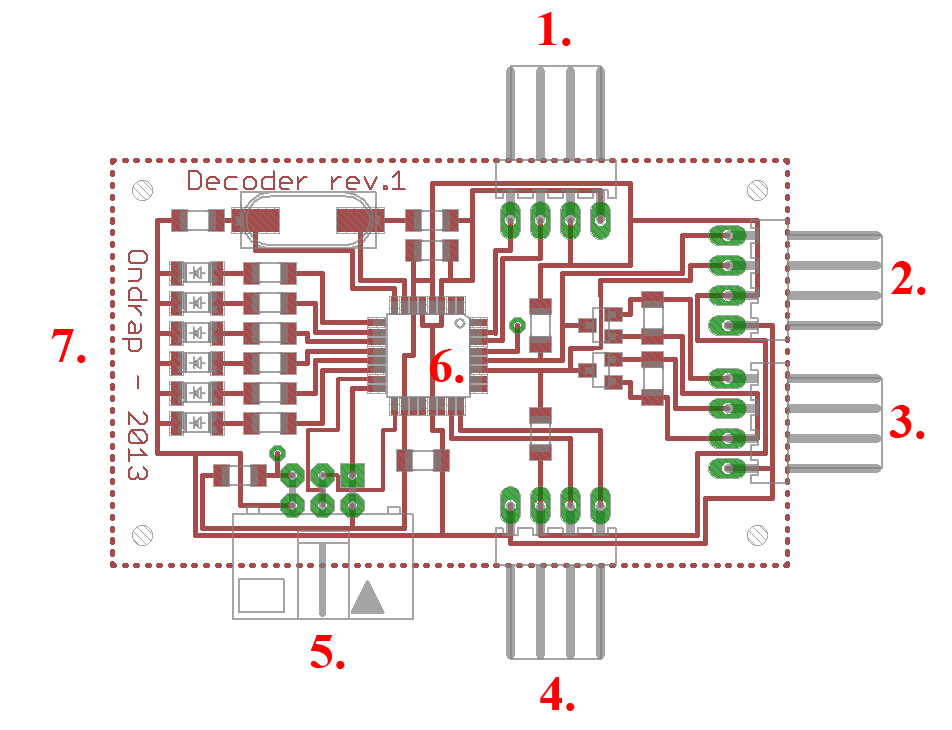
\includegraphics{dekoderyDeskaOznacena.png}
	\caption{Dekodérová deska s označením částí.}
	\label{fig:dekoderyDeska}
\end{figure}


\begin{enumerate}
	\item zámkový konektor pro připojení signálů a napájení enkodérů.
	\item zámkový konektor pro připojení 5V napájení a 5V signálů I2C.
	\item zámkový konektor pro připojení 3.3V napájení a 3.3V signálů I2C.
	\item zámkový konektor pro připojení signálů a napájení enkodérů.
	\item 6 pinový konektor ISP pro nahrávání nového programu do mikrokontroléru.
	\item mikrokontrolér Atmega48pa.
	\item diody pro indikaci stavu mikrokontroléru a jsou zapojeny na piny PB0-PB2 a PD5 - PD7.
\end{enumerate}

\newpage
\subsection{Konektory}
Deska má 2 konektory pro připojení kvadraturních enkodérů, 2 konektory pro komunikaci po I2C s 5V či 3.3V logikou a konektor ISP pro nahrávání nového kódu do mikrokontroleru.

\subsubsection{I2C konektor}
4 pinový zámkový konektor pro připojení na sběrnici I2C a napájení. Na desce jsou dva takovéto konektory s různým napětím logické 1. Jeden s 5V úrovněmi kde napájení a I2C sběrnice jsou přímo připojený na mikrokontrolér a~jeden s~3.3V úrovněmi, který je pomocí převodníku napěťových úrovní na signálech I2C připojen k 5V I2C sběrnici mikrokontroléru. U tohoto konektoru se napájecí piny používají pouze pro převodník úrovní. Zapojení jednotlivých pinů je znázorněno na obrázku \ref{fig:KonektorI2C}.
	
\begin{figure}[htbp]
	\centering
		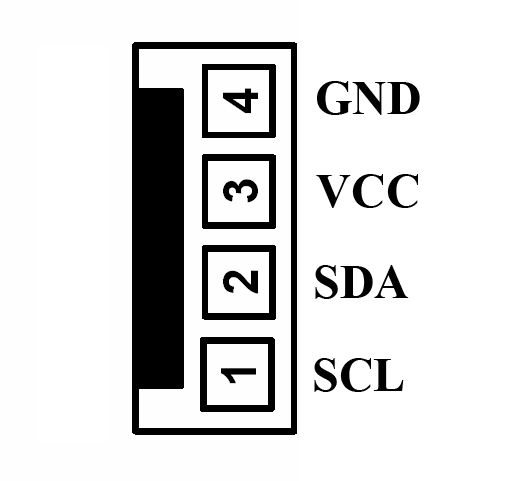
\includegraphics[scale=0.25]{KonektorI2C.png}
	\caption{Zapojení konektoru I2C.}
	\label{fig:KonektorI2C}
\end{figure}
	
\newpage	
\subsubsection{ISP konektor}
6 pinový standardní konektor pro připojení ISP programátoru jako například usbasp či PonyProg. Jednotlivé piny konektoru jsou přímo spojeny s mikrokontrolérem. Pin reset je zapojený s~pullup rezistorem 10K. Zapojení jednotlivých pinů je znázorněno na obrázku \ref{fig:KonektorISP}.

\begin{figure}[htbp]
		\centering
			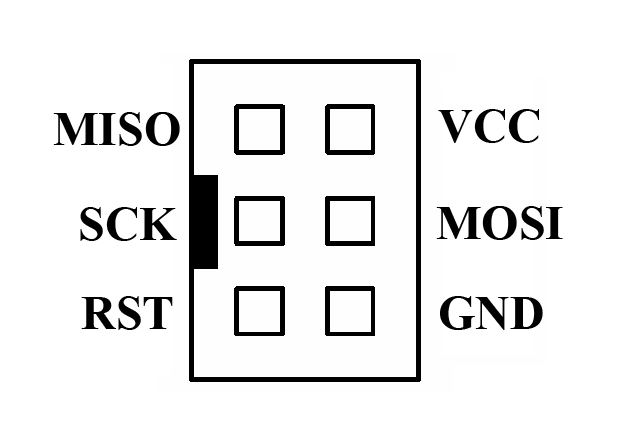
\includegraphics[scale=0.25]{KonektorISP.png}
		\caption{Zapojení konektoru ISP pro nahrávání nového kódu do mikrokontroleru.}
		\label{fig:KonektorISP}
	\end{figure}

\subsubsection{Konektor pro připojení enkodérů}
4 pinový zámkový konektor pro připojení signálů z kvadraturních enkodérů a jejich napájení. Signální piny jsou spojeny s I/O piny mikrokontroléru a napájení enkodérů je propojeno s napájením desky.

\begin{figure}[htbp]
		\centering
			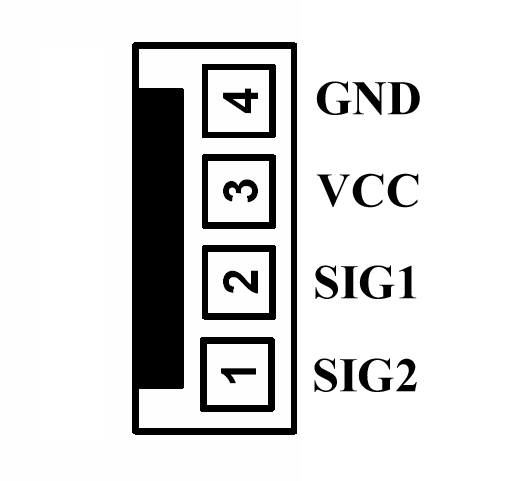
\includegraphics[scale=0.25]{KonektorEnkoder.png}
		\caption{Zapojeni konektoru pro připojení enkodérů.}
		\label{fig:KonektorEnkoder}
	\end{figure}

\newpage
\subsection{Schéma desky}
\begin{figure}[h]
	\centering
		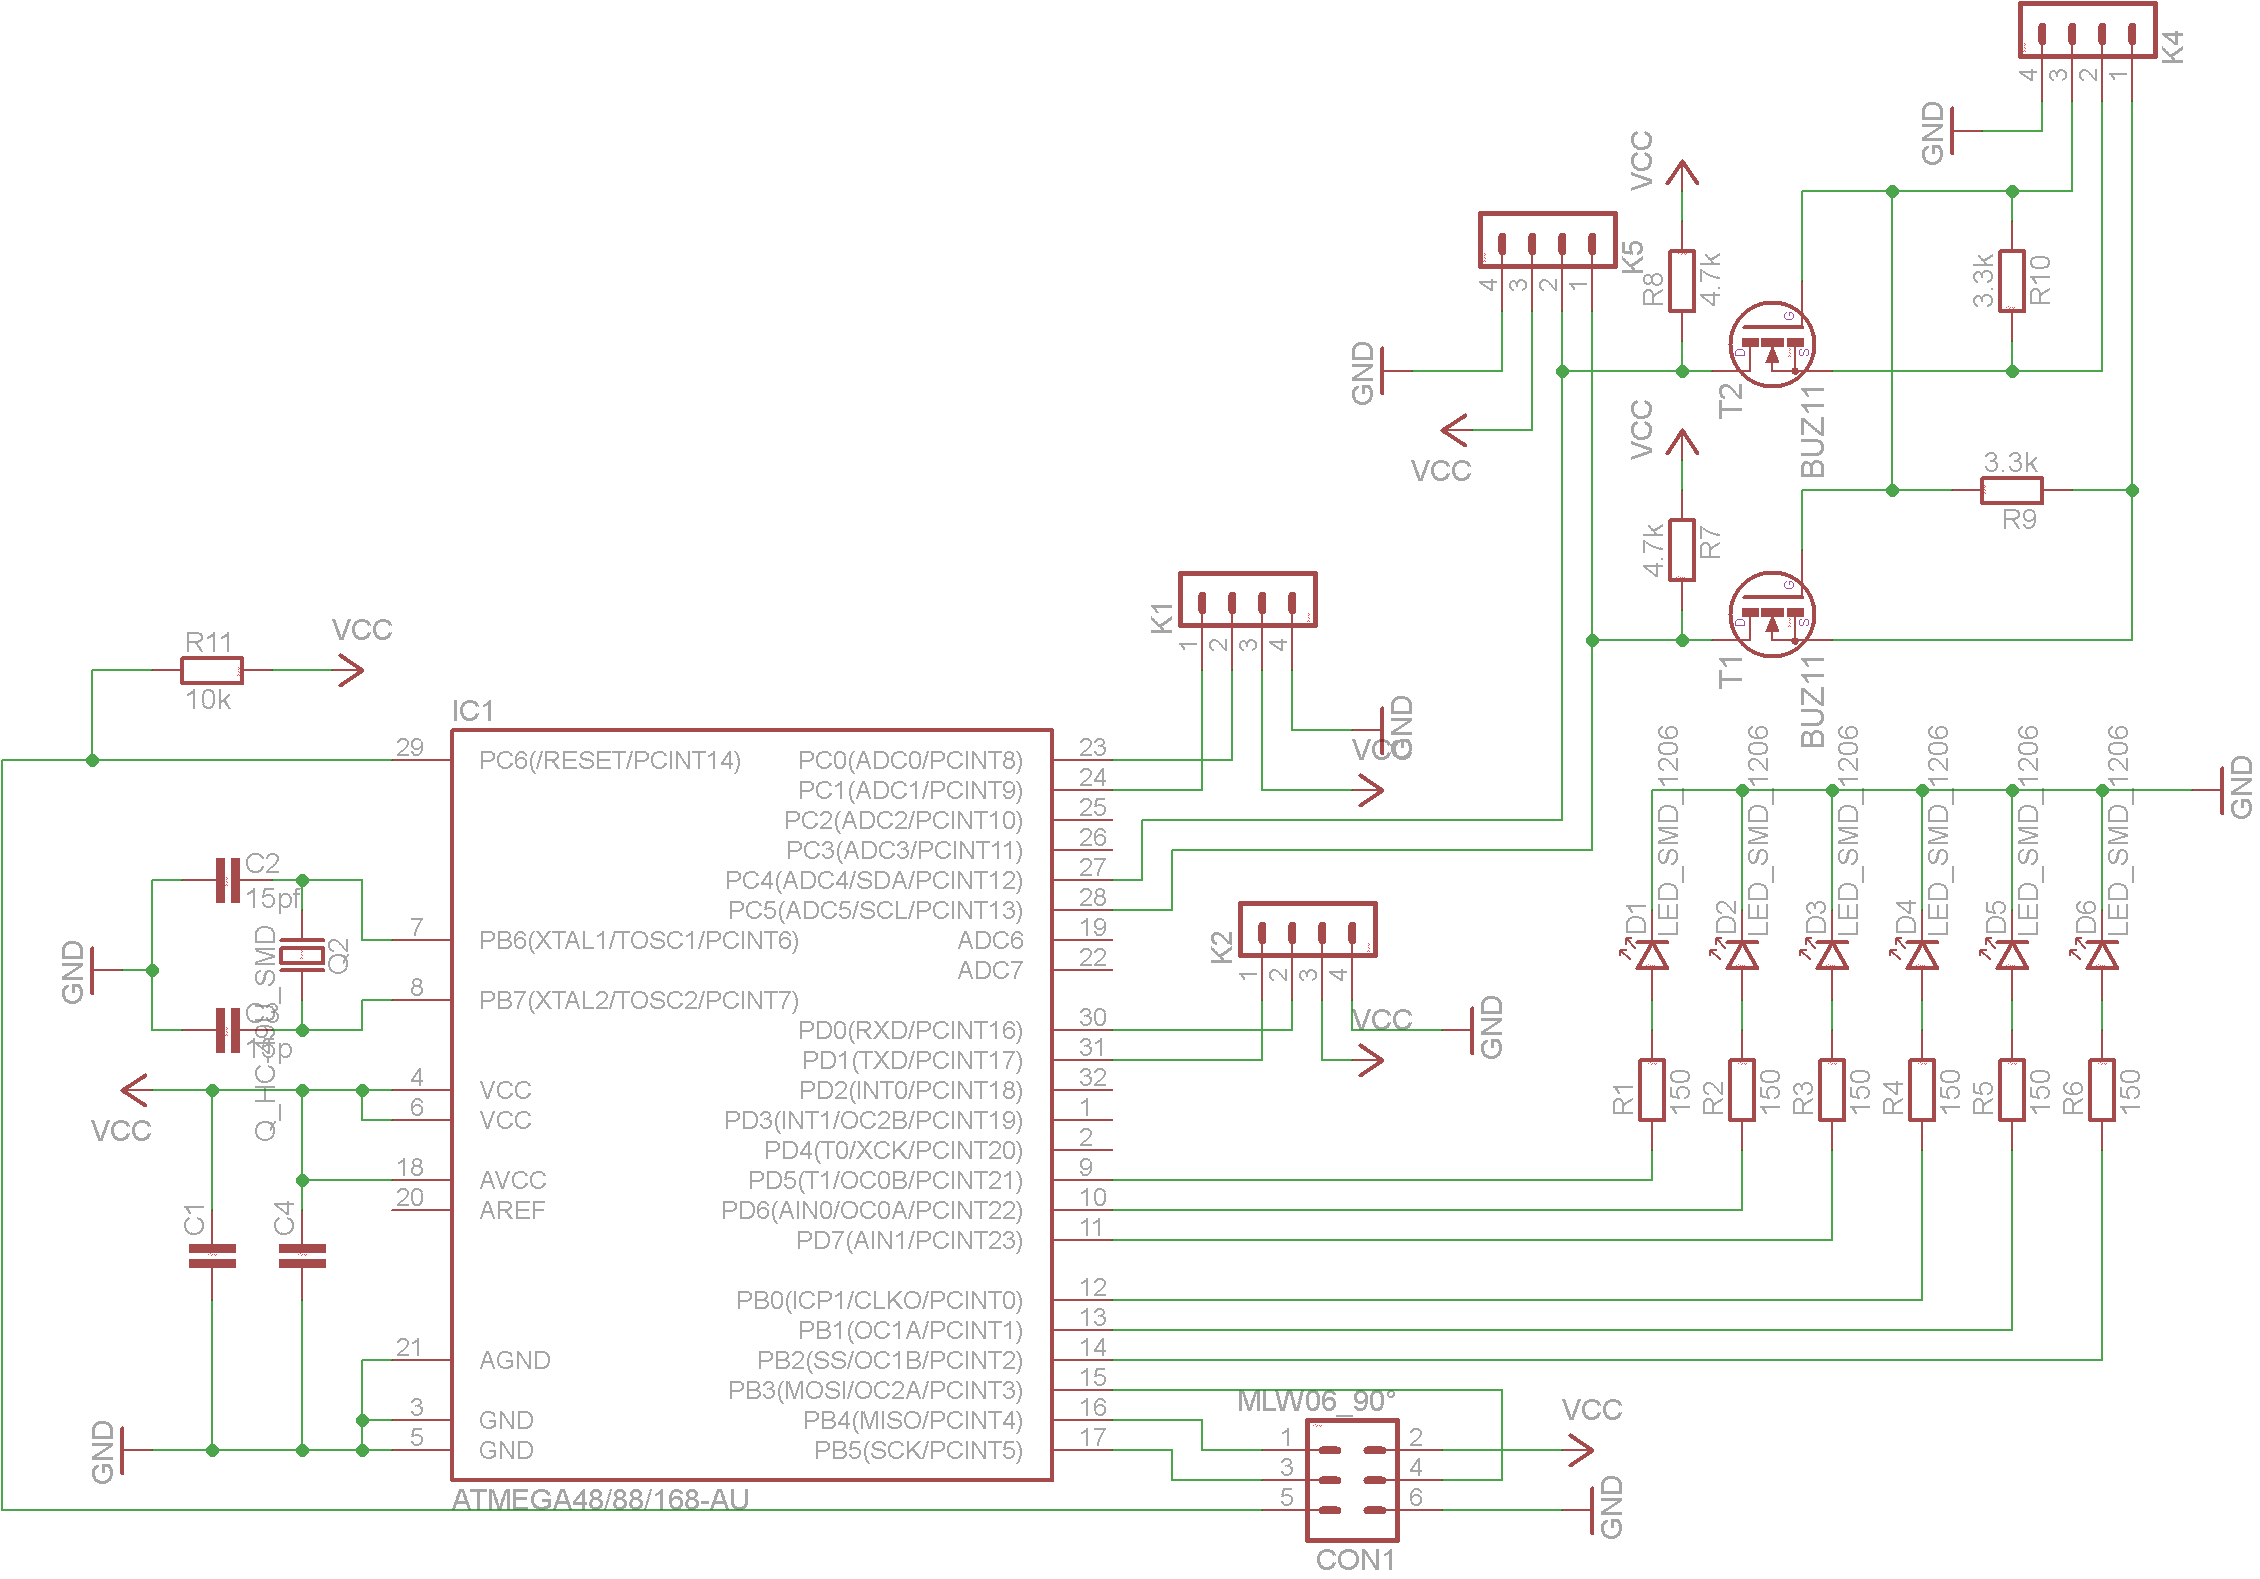
\includegraphics[scale=0.8]{dekoderySchema.png}
	\caption{Schéma dekodérové desky}
	\label{fig:dekoderySchema}
\end{figure}

\newpage
\subsection{Appendix A.}

\end{document}
